% Options for packages loaded elsewhere
\PassOptionsToPackage{unicode}{hyperref}
\PassOptionsToPackage{hyphens}{url}
\PassOptionsToPackage{dvipsnames,svgnames,x11names}{xcolor}
%
\documentclass[
  letterpaper,
  DIV=11,
  numbers=noendperiod]{scrreprt}

\usepackage{amsmath,amssymb}
\usepackage{iftex}
\ifPDFTeX
  \usepackage[T1]{fontenc}
  \usepackage[utf8]{inputenc}
  \usepackage{textcomp} % provide euro and other symbols
\else % if luatex or xetex
  \usepackage{unicode-math}
  \defaultfontfeatures{Scale=MatchLowercase}
  \defaultfontfeatures[\rmfamily]{Ligatures=TeX,Scale=1}
\fi
\usepackage{lmodern}
\ifPDFTeX\else  
    % xetex/luatex font selection
\fi
% Use upquote if available, for straight quotes in verbatim environments
\IfFileExists{upquote.sty}{\usepackage{upquote}}{}
\IfFileExists{microtype.sty}{% use microtype if available
  \usepackage[]{microtype}
  \UseMicrotypeSet[protrusion]{basicmath} % disable protrusion for tt fonts
}{}
\makeatletter
\@ifundefined{KOMAClassName}{% if non-KOMA class
  \IfFileExists{parskip.sty}{%
    \usepackage{parskip}
  }{% else
    \setlength{\parindent}{0pt}
    \setlength{\parskip}{6pt plus 2pt minus 1pt}}
}{% if KOMA class
  \KOMAoptions{parskip=half}}
\makeatother
\usepackage{xcolor}
\ifLuaTeX
  \usepackage{luacolor}
  \usepackage[soul]{lua-ul}
\else
  \usepackage{soul}
  
\fi
\setlength{\emergencystretch}{3em} % prevent overfull lines
\setcounter{secnumdepth}{-\maxdimen} % remove section numbering
% Make \paragraph and \subparagraph free-standing
\makeatletter
\ifx\paragraph\undefined\else
  \let\oldparagraph\paragraph
  \renewcommand{\paragraph}{
    \@ifstar
      \xxxParagraphStar
      \xxxParagraphNoStar
  }
  \newcommand{\xxxParagraphStar}[1]{\oldparagraph*{#1}\mbox{}}
  \newcommand{\xxxParagraphNoStar}[1]{\oldparagraph{#1}\mbox{}}
\fi
\ifx\subparagraph\undefined\else
  \let\oldsubparagraph\subparagraph
  \renewcommand{\subparagraph}{
    \@ifstar
      \xxxSubParagraphStar
      \xxxSubParagraphNoStar
  }
  \newcommand{\xxxSubParagraphStar}[1]{\oldsubparagraph*{#1}\mbox{}}
  \newcommand{\xxxSubParagraphNoStar}[1]{\oldsubparagraph{#1}\mbox{}}
\fi
\makeatother


\providecommand{\tightlist}{%
  \setlength{\itemsep}{0pt}\setlength{\parskip}{0pt}}\usepackage{longtable,booktabs,array}
\usepackage{calc} % for calculating minipage widths
% Correct order of tables after \paragraph or \subparagraph
\usepackage{etoolbox}
\makeatletter
\patchcmd\longtable{\par}{\if@noskipsec\mbox{}\fi\par}{}{}
\makeatother
% Allow footnotes in longtable head/foot
\IfFileExists{footnotehyper.sty}{\usepackage{footnotehyper}}{\usepackage{footnote}}
\makesavenoteenv{longtable}
\usepackage{graphicx}
\makeatletter
\def\maxwidth{\ifdim\Gin@nat@width>\linewidth\linewidth\else\Gin@nat@width\fi}
\def\maxheight{\ifdim\Gin@nat@height>\textheight\textheight\else\Gin@nat@height\fi}
\makeatother
% Scale images if necessary, so that they will not overflow the page
% margins by default, and it is still possible to overwrite the defaults
% using explicit options in \includegraphics[width, height, ...]{}
\setkeys{Gin}{width=\maxwidth,height=\maxheight,keepaspectratio}
% Set default figure placement to htbp
\makeatletter
\def\fps@figure{htbp}
\makeatother

\KOMAoption{captions}{tableheading}
\makeatletter
\@ifpackageloaded{tcolorbox}{}{\usepackage[skins,breakable]{tcolorbox}}
\@ifpackageloaded{fontawesome5}{}{\usepackage{fontawesome5}}
\definecolor{quarto-callout-color}{HTML}{909090}
\definecolor{quarto-callout-note-color}{HTML}{0758E5}
\definecolor{quarto-callout-important-color}{HTML}{CC1914}
\definecolor{quarto-callout-warning-color}{HTML}{EB9113}
\definecolor{quarto-callout-tip-color}{HTML}{00A047}
\definecolor{quarto-callout-caution-color}{HTML}{FC5300}
\definecolor{quarto-callout-color-frame}{HTML}{acacac}
\definecolor{quarto-callout-note-color-frame}{HTML}{4582ec}
\definecolor{quarto-callout-important-color-frame}{HTML}{d9534f}
\definecolor{quarto-callout-warning-color-frame}{HTML}{f0ad4e}
\definecolor{quarto-callout-tip-color-frame}{HTML}{02b875}
\definecolor{quarto-callout-caution-color-frame}{HTML}{fd7e14}
\makeatother
\makeatletter
\@ifpackageloaded{bookmark}{}{\usepackage{bookmark}}
\makeatother
\makeatletter
\@ifpackageloaded{caption}{}{\usepackage{caption}}
\AtBeginDocument{%
\ifdefined\contentsname
  \renewcommand*\contentsname{Table of contents}
\else
  \newcommand\contentsname{Table of contents}
\fi
\ifdefined\listfigurename
  \renewcommand*\listfigurename{List of Figures}
\else
  \newcommand\listfigurename{List of Figures}
\fi
\ifdefined\listtablename
  \renewcommand*\listtablename{List of Tables}
\else
  \newcommand\listtablename{List of Tables}
\fi
\ifdefined\figurename
  \renewcommand*\figurename{Figure}
\else
  \newcommand\figurename{Figure}
\fi
\ifdefined\tablename
  \renewcommand*\tablename{Table}
\else
  \newcommand\tablename{Table}
\fi
}
\@ifpackageloaded{float}{}{\usepackage{float}}
\floatstyle{ruled}
\@ifundefined{c@chapter}{\newfloat{codelisting}{h}{lop}}{\newfloat{codelisting}{h}{lop}[chapter]}
\floatname{codelisting}{Listing}
\newcommand*\listoflistings{\listof{codelisting}{List of Listings}}
\makeatother
\makeatletter
\makeatother
\makeatletter
\@ifpackageloaded{caption}{}{\usepackage{caption}}
\@ifpackageloaded{subcaption}{}{\usepackage{subcaption}}
\makeatother

\ifLuaTeX
  \usepackage{selnolig}  % disable illegal ligatures
\fi
\usepackage{bookmark}

\IfFileExists{xurl.sty}{\usepackage{xurl}}{} % add URL line breaks if available
\urlstyle{same} % disable monospaced font for URLs
\hypersetup{
  pdftitle={Slime Lab Manual},
  pdfauthor={David Bryan},
  colorlinks=true,
  linkcolor={blue},
  filecolor={Maroon},
  citecolor={Blue},
  urlcolor={Blue},
  pdfcreator={LaTeX via pandoc}}


\title{Slime Lab Manual}
\usepackage{etoolbox}
\makeatletter
\providecommand{\subtitle}[1]{% add subtitle to \maketitle
  \apptocmd{\@title}{\par {\large #1 \par}}{}{}
}
\makeatother
\subtitle{(aka fish / wet lab manual)}
\author{David Bryan}
\date{2026-01-05}

\begin{document}
\maketitle

\renewcommand*\contentsname{Table of contents}
{
\hypersetup{linkcolor=}
\setcounter{tocdepth}{2}
\tableofcontents
}

\bookmarksetup{startatroot}

\chapter{Introduction}\label{introduction}

(aka fish / wet lab manual)

\hfill\break

This is the \textbf{Slime Lab Manual}. This manual describes the
procedures for at sea data biological sampling and physical
oceanographic measurements that occur aboard the NOAA Ship Oscar Dyson
during a NOAA-AFSC Midwater Assessment Conservation Engineering (MACE)
survey. The manual is written to provide an overview of the sampling
procedures that take place in the chem/fish lab for new or volunteer
scientists/staff, a place for returning scientist to refresh themselves
on procedures, and in-depth guide for all tasks that occur in the slime
lab.

This manual is broken into several sections,
\href{pre-season_preparation.qmd}{Pre-Season Preparations},
\href{gear_trials.qmd}{Gear Trials}, \href{calibration.qmd}{Acoustic
Calibration}, \href{pre-haul_preparations}{Pre-Haul Preparations},
\href{sampling_procedures}{Sampling Procedures},
\href{data_verification_clams.qmd}{Data QA/QC}, and
\href{post-survey.qmd}{Post Survey Tasks}. Some
\href{references.qmd}{Additional References} are also provided. There is
a sidebar on the left to navigate to main topics. Within each topic
there is a Table of Contents on the right side of the screen that can be
used to navigate to content within that topic.

\includegraphics[width=1\textwidth,height=\textheight]{images/age1_pollock.JPG}

\section{Glossary of Terms}\label{glossary-of-terms}

Here is a \hyperref[volun-glossary]{glossary of roles and terms}
relevant to MACE surveys aboard NOAA Ships. This is helpful to anybody
new to the NOAA ship Oscar Dyson.

\bookmarksetup{startatroot}

\chapter{Pre-Season Preparation}\label{pre-season-preparation}

This is a list of tasks related to the slime lab that should be
completed before gear trials at the start of a survey season.

\section{A. Equipment Checklist}\label{a.-equipment-checklist}

Gear Inventory (MACE loading and shipping) is a rolling spreadsheet
maintained through Google Sheets to track and inventory gear shipped to
and from Alaska.
\href{https://docs.google.com/spreadsheets/d/12_39Ke-rfvQZLH6ZlejbbX5bNRX2fFNvNkkVWe21Hp8/edit?gid=1672489246\#gid=1672489246}{Click
here to open the Google Sheet}

\section{B. Special Study Supplies}\label{b.-special-study-supplies}

Pre-cruise preparation includes soliciting Special Studies requests for
all surveys during the upcoming year. In November, the MACE Special
Collections Request form is emailed to contacts on the
special\_studies\_announcement\_list which is found in the
\texttt{G:\textbackslash{}special\ studies} folder under the last survey
year. The announcement list is a living document in which new contacts
are added and old or invalid email addresses are deleted.

After they are received, Special Study requests are put in a subfolder
in \texttt{G:\textbackslash{}special\ studies} by year, then by either
Winter or Summer. Information should include: 1. Project goals with some
background information. 2. Specific sampling instructions/procedures
which include: * storage requirements. * time and space requirements. *
specific details of any activities that may impact vessel/MACE personnel
or equipment. 3. When and how supplies, chemicals, and samples will be
shipped to and from the vessel. 4. A chemical inventory.

\section{C. Sampling Requirements}\label{c.-sampling-requirements}

Obtain information on sampling requirements from stock assessment
authors. Use this to create `Table Tips'.

\begin{tcolorbox}[enhanced jigsaw, colframe=quarto-callout-note-color-frame, rightrule=.15mm, colback=white, leftrule=.75mm, arc=.35mm, breakable, bottomrule=.15mm, toprule=.15mm, left=2mm, opacityback=0]
\begin{minipage}[t]{5.5mm}
\textcolor{quarto-callout-note-color}{\faInfo}
\end{minipage}%
\begin{minipage}[t]{\textwidth - 5.5mm}

\vspace{-3mm}\textbf{📝 Draft Question: Equipment Calibration}\vspace{3mm}

Does it make sense to provide a quick run down of per-cruise
calibrations/ testing of wet lab equipment in this manual (i.e.~scales,
length boards, SBEs)?

\end{minipage}%
\end{tcolorbox}

\section{Equipment Calibration}\label{equipment-calibration}

\subsection{SBE}\label{sbe}

MACE has three \href{other\%20manuals/SBE39plusrevB.pdf}{SBE 39plus
Temperature (Depth) recorders}. These are sent in for calibration every
other year. This is typically coordinated with GAP. For years when they
are not sent in, the batteries should be replaced prior to gear trials.
They each take 4 AA 3.6V lithium batteries. To replace the batteries
unscrew the probe end. This should be possible to do by hand. Gently
pull out until the battery compartment is accessible. Try not to add
additional twists to the wires. Replace batteries and screw end back to
hand tightness.

\begin{center}
\includegraphics[width=1\textwidth,height=\textheight]{images/SBE39plus.JPG}
\end{center}

\begin{tcolorbox}[enhanced jigsaw, colframe=quarto-callout-note-color-frame, rightrule=.15mm, colback=white, leftrule=.75mm, arc=.35mm, breakable, bottomrule=.15mm, toprule=.15mm, left=2mm, opacityback=0]
\begin{minipage}[t]{5.5mm}
\textcolor{quarto-callout-note-color}{\faInfo}
\end{minipage}%
\begin{minipage}[t]{\textwidth - 5.5mm}

\vspace{-3mm}\textbf{📝 Draft Question: Age and Growth}\vspace{3mm}

Does organizing the age and growth supplies fall under this manual?

\end{minipage}%
\end{tcolorbox}

\bookmarksetup{startatroot}

\chapter{Gear Trials}\label{gear-trials}

Prior to the start of a survey season the fish and chem lab can be
set-up and equipment checked. This typically occurs during the gear
trials.

\section{A. Fish Lab}\label{a.-fish-lab}

\subsection{Equipment}\label{equipment}

If not installed already, under the direction of MACE IT unpack and
connect the \hyperref[length-boards]{length boards} and the
\hyperref[marel-scales]{Marel scales} (specimen and basket scales) at
the sampling stations and test the equipment with CLAMS.

Set up the CamTrawl battery charger in the chem lab and test both
CamTrawl units by deploying them separately on a trawl and downloading
them. Please see these pdfs for information on CamTrawl
\href{other\%20manuals/Charging\%20camTrawl\%20Batteries.pdf}{battery
charging} and the
\href{other\%20manuals/Camtrawl\%20quick\%20guide\%20Feb\%202024.pdf}{quick
guide} for operations.

During Gear Trials, do an in-water deployment test with the SBE
(temperature (depth) data recorder). See these links for directions on
SBE \hyperref[SBE-prep]{initiation} and
\hyperref[SBE-download]{downloading}.

After you've set up the fish lab (generally, during gear trials or at
the start of the summer survey), test out all the scales, length boards,
and CLAMS stations. The safest way to do this is to confirm with MACE IT
that the CLAMS active survey is `SS Fake Ship'- this ensures that test
data doesn't contaminate real survey data. Check with the IT staff to
set this up. Once you have set the CLAMS survey to SS Fake Ship, go
through a simulated haul in the fish lab (see details on standard haul
processing tasks below) remember to check all protocols are correct for
this survey including any additional protocol needs from Special Studies
(fin clips, stomachs etc.).

While not being used, store and secure the \hyperref[load-cells]{load
cells} in a dry yet accessible location like the ready room. Charge and
store the load cell batteries inside the Chem lab.

\subsection{Cheat Sheets}\label{cheat-sheets}

\begin{itemize}
\tightlist
\item
  Post Table Tips in the fish lab on inboard wall near work station 1.
\item
  Post Special Studies summaries and specific instructions and prepare
  any necessary.
\item
  Post the large MACE ID poster on the wall nearest the ready room.
\item
  Post maturity code descriptions on wall near CLAMS station 4.
\end{itemize}

\subsection{Other Gear}\label{other-gear}

\begin{itemize}
\tightlist
\item
  Set out and arrange fish lab gloves, nitrile gloves, work gloves, and
  staff raingear in the ready room area.
\item
  Set out otolith vials/caps, scalpels, tweezers, knives, pencils in a
  tub next to sink in fish lab.
\item
  Prepare oto juice - (instructions??)
\end{itemize}

\section{B. Chem Lab}\label{b.-chem-lab}

\begin{itemize}
\tightlist
\item
  Set out essential waterproof identification books and laminated id
  cheat sheets (e.g.~myctophid and jellyfish) in a location in the chem
  lab that is easily accessible.
\item
  Unpack totes of office supplies and excess fish lab sampling tools
  into drawers. Organize and label drawers by supply type for ease of
  access (e.g.~Office Supplies, Fish Lab, Bags, Tapes and Bungees etc.).
\end{itemize}

\section{C. Otoliths}\label{c.-otoliths}

Prepare Otolith supplies: Affix enough barcode labels to vials to fill
2-3 boxes. Labeled vials are arranged Left to Right, Top to Bottom (No
Zigzag) in Styrofoam trays. Write the cruise info using permanent marker
on the otolith boxes: (i.e.~- DY2401 where DY = ship name Dyson, 24 =
last 2 digits of year, 01 = cruise \#), vial barcode \# range, and the
species collected.

\section{Length Boards}\label{length-boards}

If lengths are not measuring correctly you may need to
\href{other\%20manuals/Calibrating\%20Ichthystick.pdf}{re-calibrate} the
fish length boards (caution, the ruler inlayed on the length board is
not a precise measuring tool and not used for calibration): * Place the
magnet over the clear plexiglass plate right above the green led light.
The light should turn red and then the length board should switch to
calibration mode. * The screen on the length board will display
calibration mode and it will instruct you to place the magnet at 0 cm of
the metric ruler (This should be up against the vertical barrier between
the plexiglass covered control panel and the inlayed ruler). * The
screen will then instruct you to place the magnet at 75 cm of the metric
ruler (not the ruler inlayed). The 75 cm mark is noted (in permanent
ink) on each fish board. The calibration mode will then finish and let
you know when calibration is complete.

\section{Weighing Scales}\label{marel-scales}

Locate the scale calibration weight sets in the Chem Lab floor cabinet
aft of the computers and complete a calibration followed by a
calibration test.

A scale calibration is performed by:

\begin{enumerate}
\def\labelenumi{\arabic{enumi}.}
\tightlist
\item
  Simultaneously pressing the MENU and ZERO keys:
\end{enumerate}

\begin{itemize}
\tightlist
\item
  Wait until the scale asks for a reference weight -- May take 15
  seconds. ``Put 20'' or ``Put 2'' will display.
\end{itemize}

\begin{enumerate}
\def\labelenumi{\arabic{enumi}.}
\setcounter{enumi}{1}
\tightlist
\item
  Place the reference weight (i.e.~20 or 2 kg weight) on the platform
  then press the PRINT key:
\end{enumerate}

\begin{itemize}
\tightlist
\item
  The message ``==='' appears on the display while the calibration takes
  place.
\item
  When the calibration is complete, the message ``Fit nn'' appears.
\item
  Values above 25 indicate a poor calibration; repeat calibration if
  needed.
\end{itemize}

After a calibration has been completed a calibration test should be
conducted at the start of each field season. The test weights for the
calibration test should remain stored in a dry secure location after
use. In short, the calibration test is the placement of a full range of
weights on the scale and recording the values. The scale calibration
test sheet
\href{https://docs.google.com/spreadsheets/d/1IFuS-9W8RfwYoiW8o6t_PSOgGjW957mS5xxgdI9YVB4/edit?gid=0\#gid=0}{scale
calibration test sheet} has a tab for each scale and provides a list of
the weights to be tested. The results from each scale should be
documented on its tab along with the date of the test.

\section{Load Cells}\label{load-cells}

Compare the crane scale readouts to the load cell weights. Have both
cranes (starboard and port) lift an object on the back deck. This could
be a codend or any gear. The weight read out will display in the wet lab
by clams station 1 and on the crane. Attach the loadcell and weigh the
same object, compare for accuracy. If the crane weights are not similar
to the loadcell do not use the crane readouts for fishing operations.
See section Splitter Bin Vs. Sorting Table? for safely using the
loadcell during fishing operations.

\section{SBE}\label{SBE}

The SBE should be good to go after the \hyperref[SBE]{Pre-Season
Preparations}.

\bookmarksetup{startatroot}

\chapter{Calibration}\label{calibration}

Fish lab personnel assist with acoustic calibration. If the vessel's
large CTD is not working or if staff is not available the CastAway-CTD
(aka ``football'') can be used. This piece of equipment is stored in the
Chem Lab.

\begin{tcolorbox}[enhanced jigsaw, colframe=quarto-callout-warning-color-frame, rightrule=.15mm, colback=white, leftrule=.75mm, arc=.35mm, breakable, bottomrule=.15mm, toprule=.15mm, left=2mm, opacityback=0]

\textbf{More Info Needed:} I am thinking some instructions on the
calibration spheres and downriggers would be nice.

\end{tcolorbox}

\section{CastAway-CTD}\label{castaway-ctd}

For select purposes the CastAway-CTD can be used as alternative to the
large CTDs. The larger CTD may require 3-4 ship crew to safely cast over
the ``Hero deck'' (side sampling station) while the small football CTD
only requires 1 individual. To cast the CastAway-CTD secure it to the
railing on the ``Hero deck'' and lower down to 30m. Communicate with the
Bridge before and after lowering anything into the water from the ship.

\begin{enumerate}
\def\labelenumi{\arabic{enumi}.}
\tightlist
\item
  If not installed, insert two of the rechargeable AA batteries included
  in the CastAway case into the CT
\end{enumerate}

\begin{enumerate}
\def\labelenumi{\alph{enumi}.}
\tightlist
\item
  Remove the rubber outer case and unscrew bottom end cap to insert
  batteries, then reinsert CTD into rubber outer case
\end{enumerate}

\begin{enumerate}
\def\labelenumi{\arabic{enumi}.}
\setcounter{enumi}{1}
\tightlist
\item
  Using the magnetic stylus, turn on the CTD by inserting the magnetic
  end of the stylus into the contact on the top left of the screen.
\item
  Using the contact on the bottom left to move the selection (white
  box), make sure the deployment symbol , the small image of the CTD, is
  selected.
\item
  To start the cast, touch the contact on the bottom right with the
  magnetic stylus. The CTD will report if it is still waiting for GPS
  signal which is required for the date /time.
\item
  After the cast is complete, touch the contact on the bottom right
  again to end the recording.
\end{enumerate}

\href{other_manuals/CastAway\%20CDT\%20Users\%20Manual.pdf}{CastAway CTD
Manual}

\begin{center}
\includegraphics[width=0.5\textwidth,height=\textheight]{images/castaway.png}
\end{center}

\bookmarksetup{startatroot}

\chapter{Pre-Haul Preparation}\label{pre-haul-preparation}

It is the responsibility of the Chief Scientist or their designee to
determine the areas/depths where trawl hauls will be made. Decisions
will be based on a semi-systematic, opportunistic sampling scheme to
maximize the value of each sample with respect to the objectives of the
survey. Once the timing of sampling has been determined there are
several items that can be prepared in the fish lab.

\begin{itemize}
\tightlist
\item
  Check with FPC or Cave lead to see if you are needed for the
  \hyperref[whale-watch]{whale watch}
\item
  Initiate the \hyperref[SBE-prep]{SBE} and hang outside fish lab
\item
  Prepare the \hyperref[camtrawl]{Camtrawl} with a charged battery,
  ensure that green light is slowly blinking and place at fish lab
  entrance
\item
  Calibrate \hyperref[marel-scales]{Marel scales}
\item
  Check that all \hyperref[sampling-supplies]{sampling supplies} are
  refilled and replaced as needed
\end{itemize}

\section{SBE}\label{SBE-prep}

Trawls and Methots will be equipped with an SBE, commonly referred to as
the ``pipe bomb''. These data provide a temperature at depth profile
from which an average headrope depth and an average headrope temperature
are calculated. As part of the pre-haul preparations, the SBE needs to
be set to record.

\begin{enumerate}
\def\labelenumi{\arabic{enumi}.}
\tightlist
\item
  To connect to the SBE make sure it is plugged into the 4-pin connector
  correctly. The cable and SBE is located above the fish lab sink. Open
  the SBE Downloader on Workstation 3.
\end{enumerate}

\begin{center}
\includegraphics[width=0.5\textwidth,height=\textheight]{images/sbe_downloader.png}
\end{center}

\begin{enumerate}
\def\labelenumi{\arabic{enumi}.}
\setcounter{enumi}{1}
\tightlist
\item
  Once the downloader program is open, click on ``connect''. At the
  deployment of a haul it does not matter what haul number is displayed,
  however, following a haul you should start CLAMS at workstation 1 and
  initiate the current haul processing prior to opening the SBE
  Downloader to ensure that the SBE data are logged to the correct haul.
\end{enumerate}

\begin{center}
\includegraphics[width=0.5\textwidth,height=\textheight]{images/sbe_downloader_II.png}
\end{center}

\begin{enumerate}
\def\labelenumi{\arabic{enumi}.}
\setcounter{enumi}{2}
\tightlist
\item
  The dialog box will scroll through some text. Once the dialog box
  stops, click on ``start logging''.
\end{enumerate}

\begin{center}
\includegraphics[width=0.5\textwidth,height=\textheight]{images/sbe_downloader_III.png}
\end{center}

\begin{enumerate}
\def\labelenumi{\arabic{enumi}.}
\setcounter{enumi}{3}
\tightlist
\item
  A dialogue box will pop up asking if you are sure that you want to
  start logging which will clear all data currently on the device. This
  will reset the sample number to 0 and begin logging data after you
  click OK.
\end{enumerate}

\begin{center}
\includegraphics[width=0.5\textwidth,height=\textheight]{images/sbe_downloader_IV.png}
\end{center}

\begin{enumerate}
\def\labelenumi{\arabic{enumi}.}
\setcounter{enumi}{4}
\tightlist
\item
  Let the program run until you can see that the SBE is logging data
  every 3 seconds. Then click on ``Done''. This will quit the SBE
  downloader and you can unplug the SBE cable and put the rubber dummy
  plug on. Place the SBE for the deck crew to mount to the net.
\end{enumerate}

\begin{center}
\includegraphics[width=0.5\textwidth,height=\textheight]{images/sbe_downloader_V.png}
\end{center}

\section{CamTrawl}\label{camtrawl}

Ensure a
\href{other\%20manuals/Charging\%20camTrawl\%20Batteries.pdf}{charged
CamTrawl battery} is placed in the CamTrawl, connected, closed, and
secured with a ``spaghetti'' locking cord. Verify that the green light
is slowly blinking on the dummy plug before deck crew attaches the
assembly to the net. Floats should be upright or to the port side if
laying down on top of the net The deck crew is responsible for securing
the CamTrawl to the net. For more information see the latest CamTrawl
\href{other\%20manuals/Camtrawl\%20quick\%20guide\%20Feb\%202024.pdf}{quick
guide}.

\begin{center}
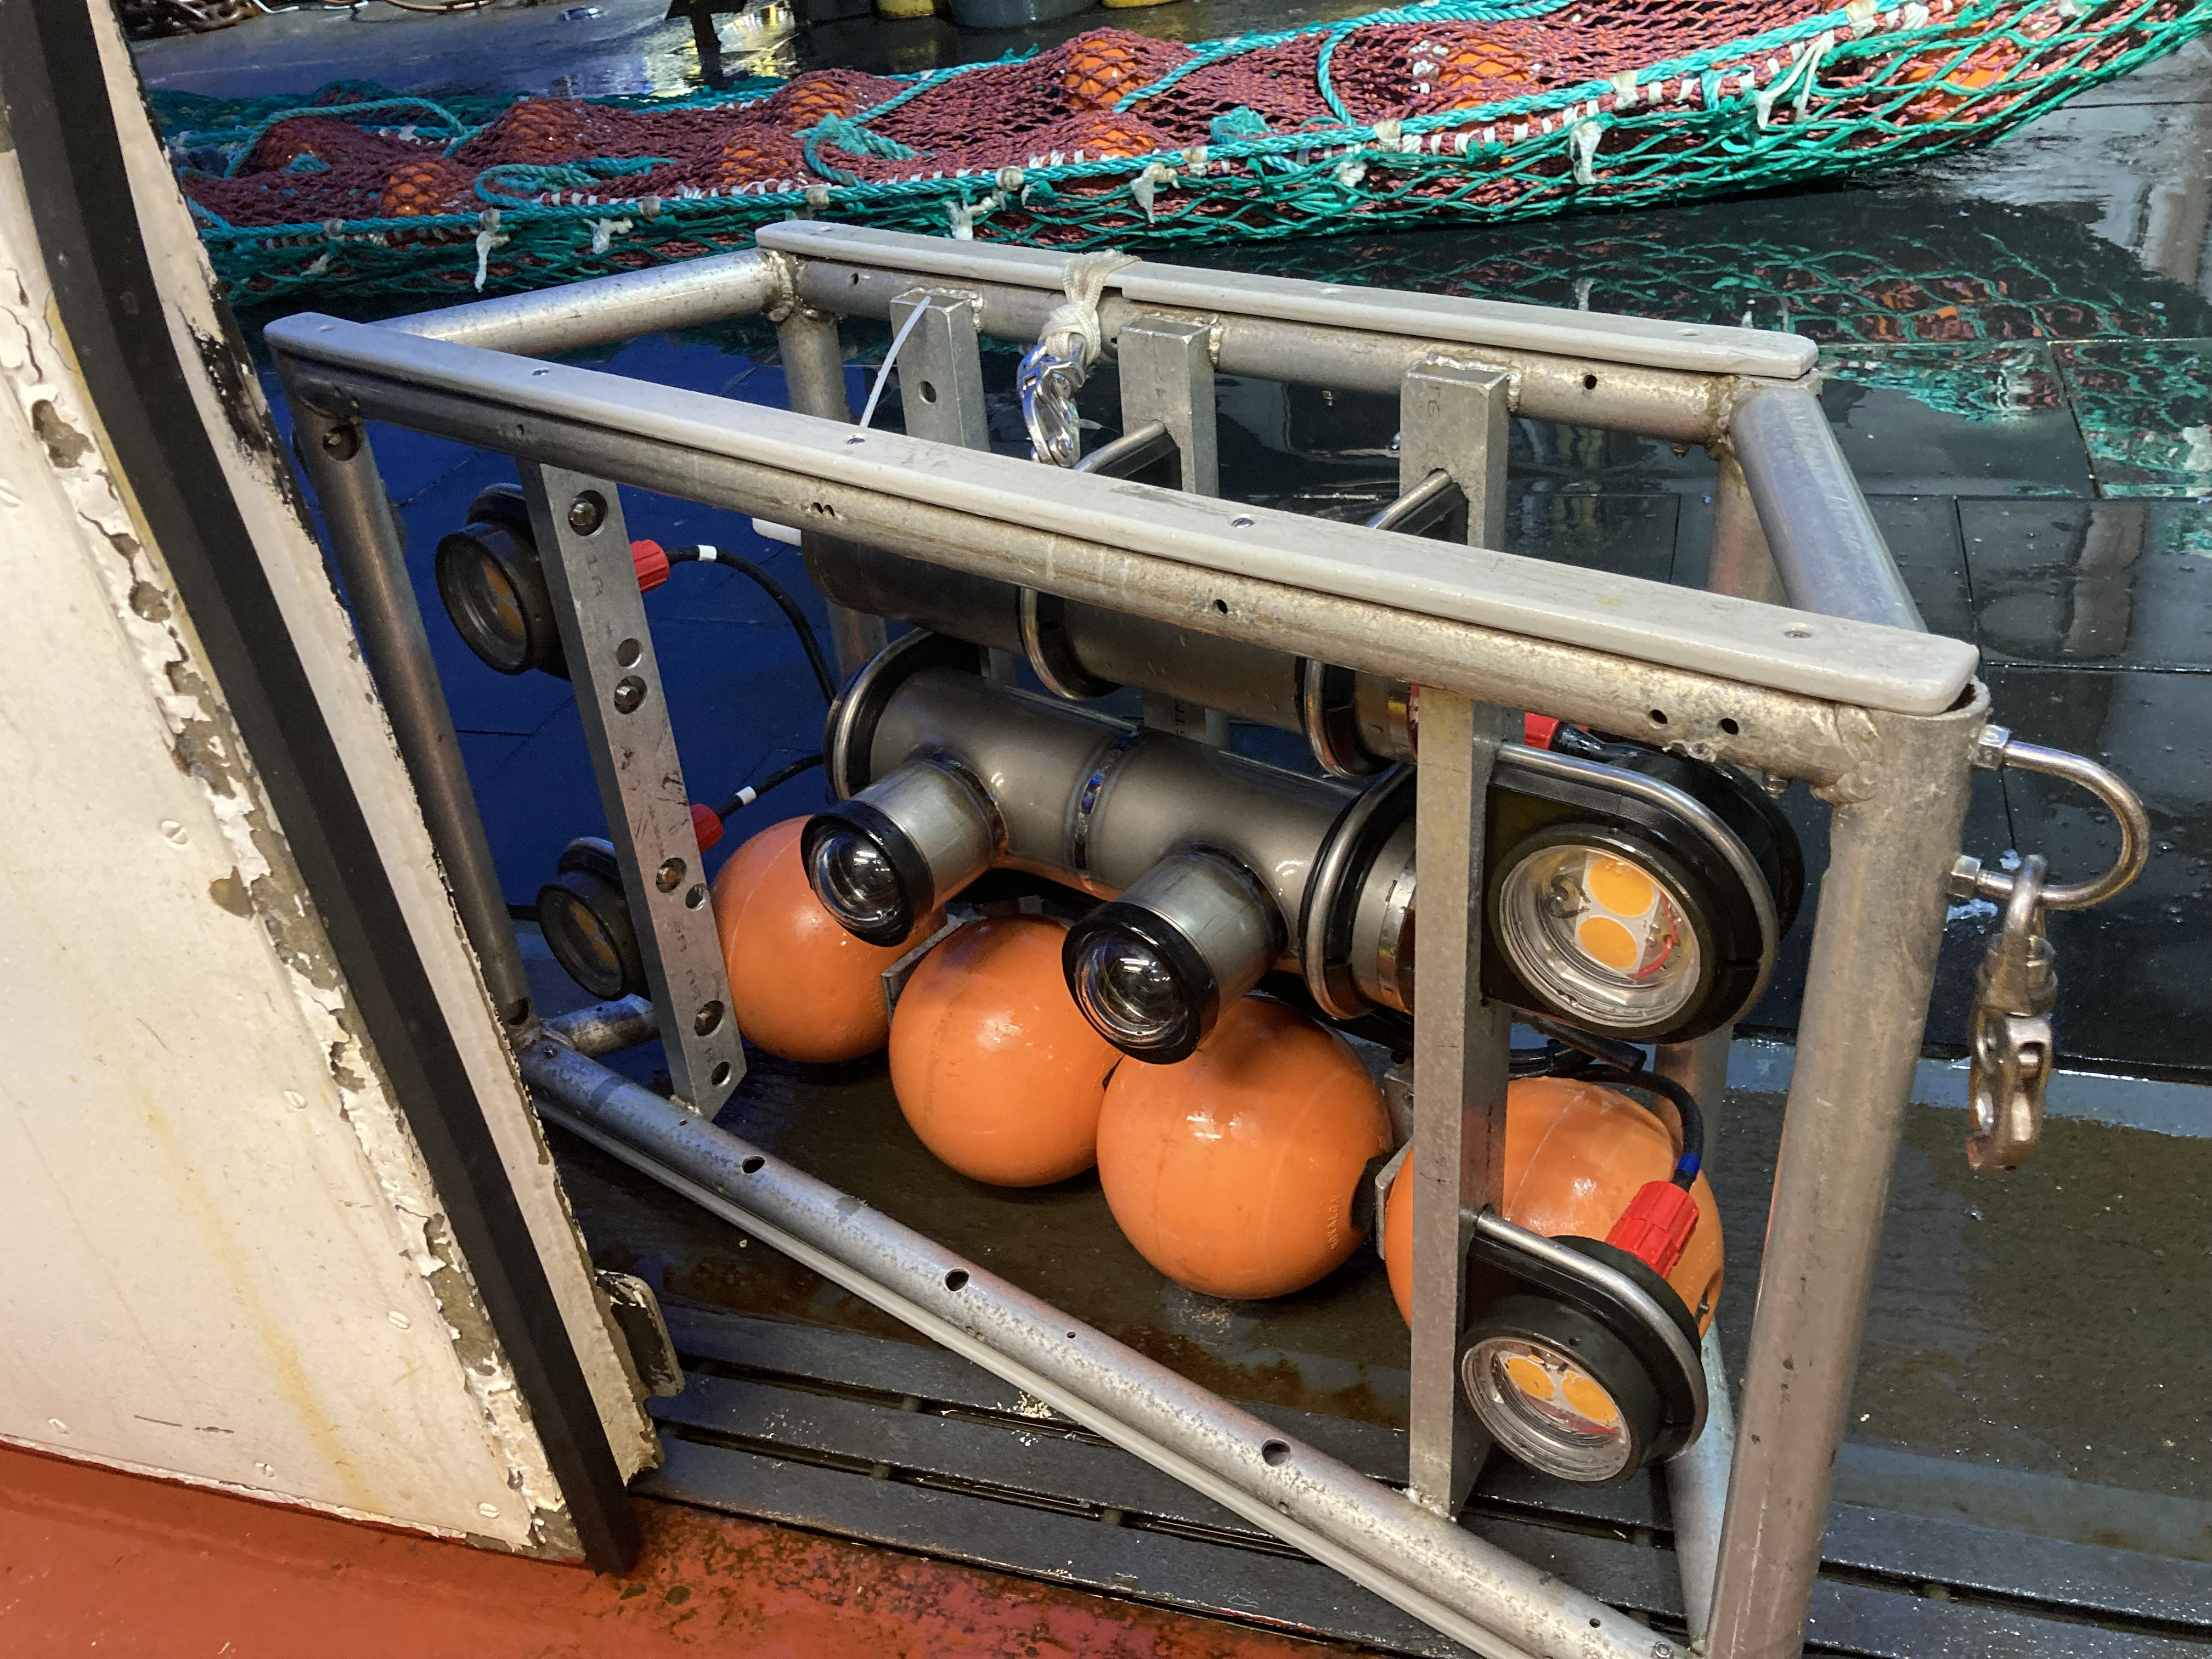
\includegraphics[width=1\textwidth,height=\textheight]{images/camtrawl.jpg}
\end{center}

\section{Marel Scales}\label{marel-scales}

The large basket scale (at the end of the conveyor belt) and the smaller
specimen scales (on the counters) require calibration before each haul
is processed - use the stainless steel 20 kg (large scale) and 2 kg
(small scale) weights provided for this purpose for each scale
respectively. Remove all objects from scale and dump any water collected
on top the 20 kg weight.

\textbf{Marel M1100 Calibration:}

\begin{enumerate}
\def\labelenumi{\arabic{enumi}.}
\tightlist
\item
  Simultaneously press the MENU and ZERO keys:
\end{enumerate}

\begin{itemize}
\tightlist
\item
  Wait until the scale asks for a reference weight -- May take 15
  seconds. ``Put 20'' or ``Put 2'' will display.
\end{itemize}

\begin{enumerate}
\def\labelenumi{\arabic{enumi}.}
\setcounter{enumi}{1}
\tightlist
\item
  Place the reference weight (i.e.~20 or 2 kg weight) on the platform
  then press the PRINT key:
\end{enumerate}

\begin{itemize}
\tightlist
\item
  The message ``==='' appears on the display while the calibration takes
  place.
\item
  When the calibration is complete, the message ``Fit nn'' appears.
\item
  Values above 25 indicate a poor calibration; repeat calibration if
  needed.
\end{itemize}

\textbf{Notes:}

\begin{itemize}
\tightlist
\item
  While using the scale, Grade should be selected not Packing. Use the
  up or down arrow to change. The scale will not input weight into Clams
  when in Packing mode.
\item
  Place an empty basket or tub on the scale and press ``Tare''. You are
  ready to weigh baskets!
\item
  If the scale is not providing steady readings and it has become
  difficult to collect weights, it may be necessary to re-calibrate
  scales mid-haul. This can occur if the weather changes or the ride of
  the ship changes between the initial calibration and getting back on
  transect.
\item
  If the scale can not provide readings and the measuring plate appears
  loose and moves independently of the base. The load cell bolts may be
  loose and require tightening. There are two sets on either side of the
  scale.
\end{itemize}

\begin{center}
\includegraphics[width=0.75\textwidth,height=\textheight]{images/marel_scale_load_cell_bolts.png}
\end{center}

\section{Sampling Supplies}\label{sampling-supplies}

Replace and refill standard sampling supplies such as scalpel blades,
the glycerol thymol squeeze bottle, vials caps, and the otolith vials
trays as needed.

Determine if special study requests are applicable for the region and
haul type and prepare for sampling if necessary (i.e., set up supplies,
prepare labels, ovary bags, storage bags).

\section{Protected Species Watch (AKA Whale Watch)}\label{whale-watch}

\includegraphics[width=1\textwidth,height=\textheight]{images/orcas.jpg}

Check in the with FPC or Cave Lead to determine if you are requested to
complete a whale watch on the bridge 15 minutes prior to the net
entering the water. Updated protocols for protected species observation
and avoidance measures is located in the ``BOC Associated Documents''
folder or the current cruise folder. For 2025, look for the document
titled ``MACE protected species at-sea procs\_FY25\_v11.docx''. When
beginning whale watch a common practice is to check in with the Officer
on Deck (OOD) and ask if they have seen any protected species near the
fishing location and what direction the ship will be heading for
fishing. Observations for protected species can be focused in that
direction.

\bookmarksetup{startatroot}

\chapter{Sampling Procedures}\label{sampling-procedures}

This section of the manual provides instruction on what to when a
midwater or bottom trawl catch first comes
\hyperref[recording-catch]{onboard}, how to sort the catch on the
\hyperref[slime-line]{slime line}, and how to collect
\hyperref[bio-samps]{biological samples}. There is also a section on how
to handle \hyperref[methots]{Methot trawls}.

\section{Saftey and Ergonomics}\label{saftey-and-ergonomics}

Prior to beginning sampling, take time to consider physical saftey and
ergonomics. There are several steps that can be taken.

\begin{itemize}
\tightlist
\item
  Consider some pre sampling stretches to warm up muscles (link to GAP
  stretches).
\item
  The fish lab is wet and slippery, make sure that the non-slip floor
  mats are placed at all workstations.
\item
  Remember to limit basket weights to 20 kg to prevent injuries and
  practice safe \hyperref[lifting]{lifting techniques}.
\item
  use two people to move heavy objects like the camtrawl or large totes
  of fish from the deck.
\end{itemize}

\section{Midwater or Bottom Trawl catches}\label{recording-catch}

\subsection{1. Recording the catch in
CLAMS}\label{recording-the-catch-in-clams}

Open the Catch Logger for Acoustic Midwater Surveys (CLAMS) app; See the
document CLAM Digging located in the folder
\texttt{G:\textbackslash{}CLAMS} for entering catch data on the CLAMS
app.

\begin{tcolorbox}[enhanced jigsaw, colbacktitle=quarto-callout-caution-color!10!white, rightrule=.15mm, toptitle=1mm, breakable, bottomrule=.15mm, coltitle=black, colframe=quarto-callout-caution-color-frame, title=\textcolor{quarto-callout-caution-color}{\faFire}\hspace{0.5em}{CLAMS}, colback=white, opacitybacktitle=0.6, arc=.35mm, left=2mm, bottomtitle=1mm, titlerule=0mm, toprule=.15mm, leftrule=.75mm, opacityback=0]

The CLAM digging document in G is from 2013. Is there some updated
instructions somewhere that we can reference? Any quick bullets we could
add here?

\end{tcolorbox}

\subsection{2. Equipment Retrieval}\label{equipment-retrieval}

As the net is hauled back, obtain the SBE from the deck crew and
\hyperref[SBE-download]{download} it as soon as possible. The SBE
downloader app is located on the forward computer nearest the sink.

Rinse the CamTrawl with fresh water and if time allows
\href{other\%20manuals/Camtrawl\%20quick\%20guide\%20Feb\%202024.pdf}{download}
the images before the next deployment.

It is common for other equipment to be handed over to the slime lab from
the deck crew; various integrated trawl instrumentation (ITI) and
special study instrumentation (light sensors, etc.).

\subsection{3. Splitter Bin Versus Sorting
Table}\label{splitter-bin-versus-sorting-table}

Catches with a total catch weight of less than \textasciitilde{} 2,000
kg (2 tons) can be dumped directly into the sorting table (link to that
section) However, for larger catches (\textgreater2,000 kg) they must
first go into a deck ``splitter'' bin and are ``split'' for a subsample.

\begin{center}
\includegraphics[width=1\textwidth,height=\textheight]{images/splitter.jpg}
\end{center}

\subsection{4. Splitter Bin}\label{splitter-bin}

\begin{itemize}
\item
  For split catches, a total catch weight must be obtained by weighing
  the catch in the codend. The load cell(provide link to instructions)
  or the crane scale may be used. Each (?) crane has an internal scale
  that has a readout both at the crane and in the fish lab. However the
  crane scales and/or the readout in the fish lab is not always
  reliable. A weight from the load cell is preferred.
\item
  Once the load cell is secure and hanging from the crane hook press
  TARE and you are ready to weigh the codend.
\item
  After the codend is weighed and recorded the catch is dumped into the
  deck ``splitter'' bin.
\item
  Next the the weight of the empty codend should be recorded.
\item
  A cargo (brailer) net attached to a metal frame in the bottom of the
  splitter bin is used to collect a subsample of the catch. This
  subsample is then lifted into the sorting table.
\item
  Once the crane is secure, wear PPE and receive deck permission to
  check the sorting table and splitter bin to make sure the catch is
  representative/homogenous.
\item
  The total catch weight is the difference of the full codend and the
  weight of the empty codend. The load cell can output in either pounds
  or kilograms. Make sure the load cell reads in kilograms, otherwise
  select the pounds unit in CLAMS.
\end{itemize}

\textbf{Splitter Tips}

\begin{itemize}
\item
  If getting weights from the load cell on deck, checking the splitter
  bin, or checking the sorting table make sure you are wearing PPE
  (helmet + floatation, either a float coat or life jacket)! Also make
  sure the deck crew know you are out there.
\item
  Deleted a note about using Whole Haul here. I think the practice of
  doing that is discouraged. Maybe want to double check that whole haul
  sampling for a single species is described somewhere, for example in
  case of a shark.
\item
  If the total catch exceeds the capacity of the deck ``splitter'' bin
  and the catch is not homogenous, splits should be repeated (with
  subsequent emptying of the bin) until the entire codend is empty.
  Alternately, the end of the codend has been pinched off at the thick
  strap and placed into the sorting table and the rest of the catch
  dumped overboard. This is not ideal but has happened due to excessive
  catch, poor weather conditions, and inexperienced crew preventing safe
  splitter bin operations.
\end{itemize}

\subsection{Shark or Marine Mammal}\label{shark-or-marine-mammal}

If a large shark is caught please follow the
\href{other\%20manuals/Shark_protocol_20230428.pdf}{MACE protocol} for
its release. Remember to collect \_\_\_ measurements if possible.

Follow the marine mammal protocol (?) if one is caught.

\section{Slime Line}\label{slime-line}

The catch from the sorting table flows directly onto the `slime line'
though a hydraulic door.

\begin{center}
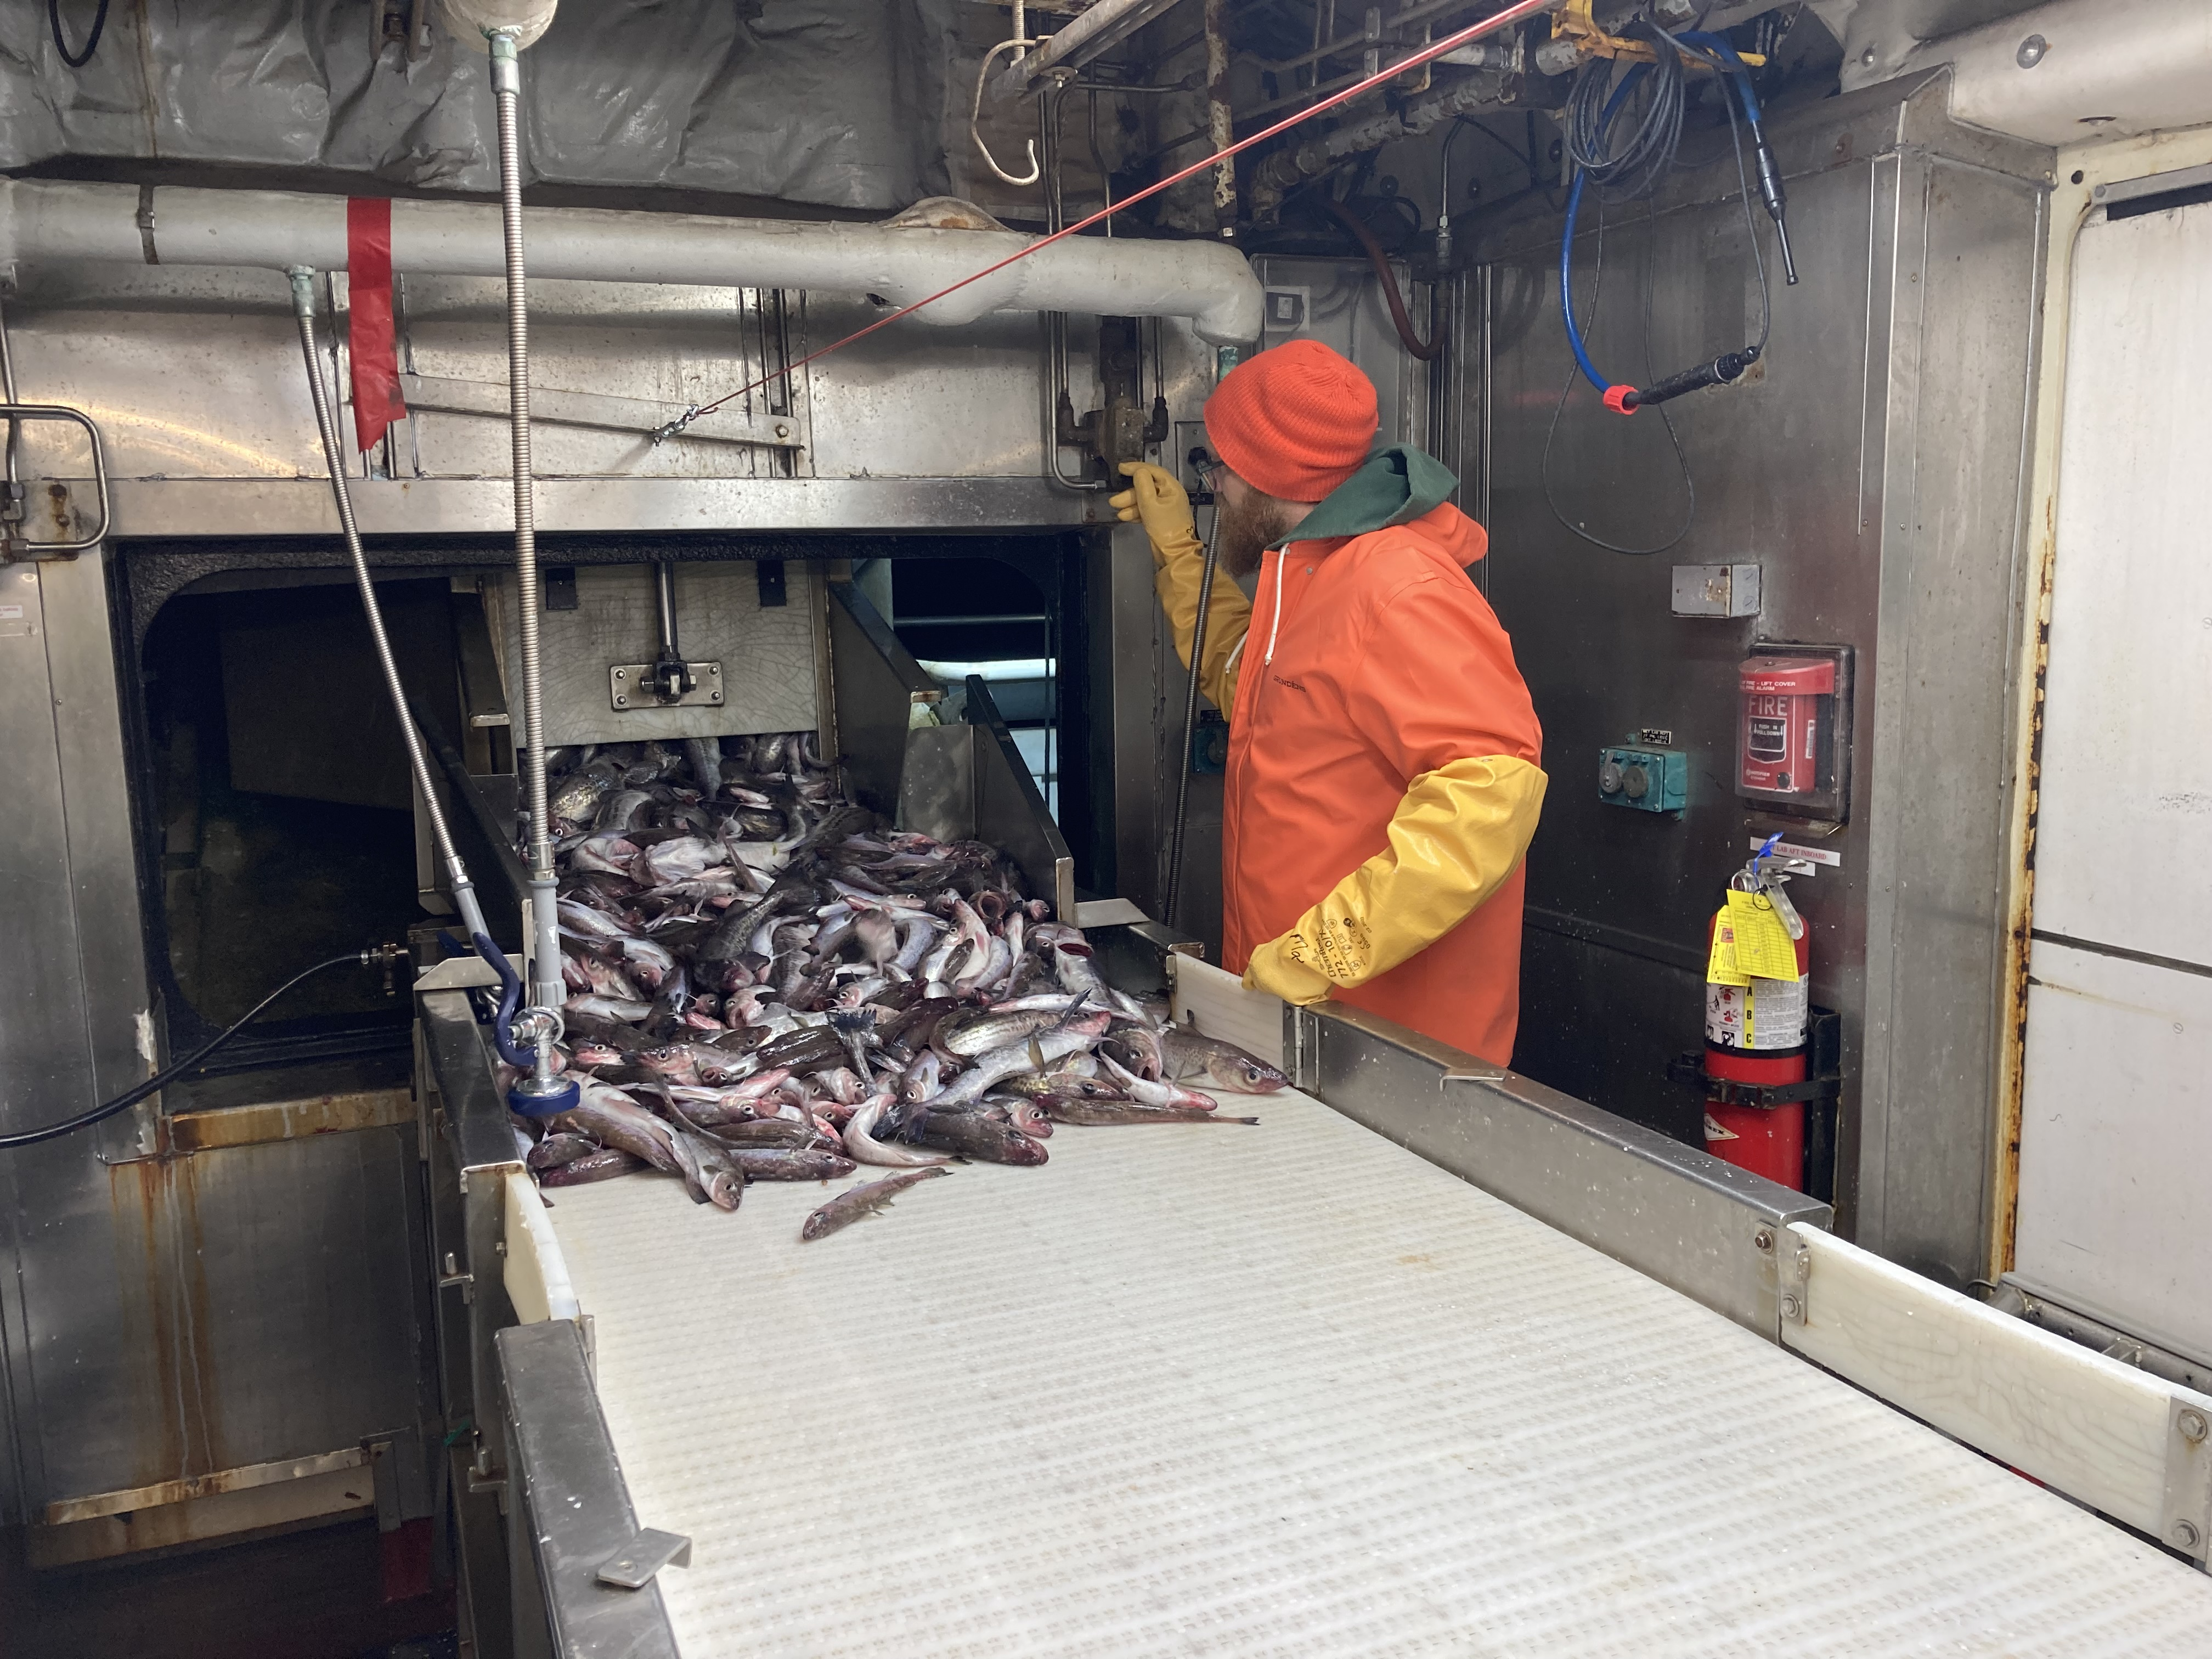
\includegraphics[width=1\textwidth,height=\textheight]{images/fish_on_belt.jpg}
\end{center}

\subsection{Roles}\label{roles}

At least three people are desirable for the slime line. One person
(often the Fish Lab Lead) operates the belt system and also weighs and
enters the catch data into CLAMS. It is essential for this person to be
following the ``Table Tips'' for species collection intended for length
frequency measurements, biological sampling, and Special Studies for the
current survey. Table Tips are updated for each winter and summer
survey, particularly biological collections and Special Studies. The
second person operates the hydraulic sorting table door using the lever
on the inboard side of the sorting belt (see image above) and allows the
catch to steadily and slowly flow from the sorting table to the sorting
belt so the catch can be efficiently screened and sorted by the slime
line team. The third person will also sort species from the belt as
directed by the Fish Lab Lead and often stands on the outboard side of
the sorting belt. If there is low bycatch and the catch requires minimal
sorting, only 2 people are necessary to run the slime line. In this
case, the third person may get a jump start on measuring the lengths of
the target species set aside by the Fish Lab Lead. If bycatch composes a
significant portion of the catch, the third person helps sort out items
from the catch to be weighed and measured after the table has been
emptied.

\subsection{Operations}\label{operations}

Once the deck area around the sorting table is clear of deck operations
and the ok is given from the deck lead, the sorting table can be raised.
Clearly shout out to the deck ``Table coming up!'' so they are aware and
the person on the outboard side of the sorting belt can raise the table
using the hydraulic lever. The catch is steadily and slowly dumped onto
the sorting belt by raising and lowering the table door to maintain a
single layer of fish on the table that can be sorted through. The catch
is sorted by species and weighed.

Once some of the catch has been allowed to flow onto the sorting belt,
pause and make a sampling strategy! Reference common sampling strategies
(i.e.~the `sorting pollock' table tips slide) and consider suggestions
from team members; they may have an alternative, more efficient sorting
strategy. Once a strategy has been chosen confirm it with the fish lab
team so everyone is on the same page working together.

\begin{itemize}
\item
  Remember to avoid ``picking'' species or pollock of a particularly
  large or small size class from the belt unless you pick ALL
  individuals of that species/size or subclass of that species.
\item
  When hauls are composed almost entirely of one species, the bycatch
  can be sorted off the sorting belt while the dominant species is left
  on the belt to be load into baskets and weighed. For example, all non
  dominant species are placed into a bin to be sorted after the belt is
  cleared.
\item
  Occasionally there are 2 predominant species in the catch such as
  pollock and jellyfish, pollock and POP, or even pollock and a Mix. It
  is more ergonomic to leave both species on the belt and sort the 2
  predominant species by sliding/tossing one species forward while
  leaving the other behind. This creates an alternating flow of two
  species moving towards the scale. The person at the scale weighing the
  catch will then need to switch between the two species in CLAMS while
  recording weights.
\end{itemize}

\begin{tcolorbox}[enhanced jigsaw, colframe=quarto-callout-note-color-frame, rightrule=.15mm, colback=white, leftrule=.75mm, arc=.35mm, breakable, bottomrule=.15mm, toprule=.15mm, left=2mm, opacityback=0]
\begin{minipage}[t]{5.5mm}
\textcolor{quarto-callout-note-color}{\faInfo}
\end{minipage}%
\begin{minipage}[t]{\textwidth - 5.5mm}

When weighing baskets of selected species at the end of the sorting belt
be mindful of the weight of the baskets. Repetitive heavy lifting of
full baskets is discouraged at sea and may result in ``repetitive
stress/strain injuries.'' Consider maintaining a maximum basket weight
of \textasciitilde20kg. It is encouraged to set aside \textbf{more}
baskets that are \textbf{lighter} to make the lifting easier and
\textbf{safer} for the fish lab \textbf{team}.

\end{minipage}%
\end{tcolorbox}

A reminder that \ul{everything in the catch gets weighed}, then it is
designated as being Measured, Counted or Tossed. Baskets that are
retained for length/sex or biological sampling are designated
``Measure''. Baskets that are weighed and ``Tossed'' are tossed over
through the discard shoot. Baskets of target species are generally not
``Counted'', this is typically reserved for catch species that we do not
length (amphipods) or abundant larval fish such as Age-0 pollock.
``Count'' baskets may be discarded after the counted amount has been
entered into CLAMS.

Digital species ID guides for
\href{other\%20manuals/FishGuide2024_03_06.pdf}{Fishes} and
\href{other\%20manuals/invert_guide_vol1.pdf}{Invertebrates} can be
accessed by clicking on the links. A suite of hard copies of ID guide
books can also be found in the Chem Lab.

\subsection{Subsample selection}\label{subsample-selection}

Since weighing and measuring all individuals that have been sorted on
the belt is not typically feasible (except for small hauls), a subsample
of predominate species or species mixes is made. Subsamples can be taken
from the targeted catch (often pollock or POP) and from the bycatch
(everything else; often forage fishes). When the catch is subsampled, it
must be random and representative of the whole catch.

When taking a subsample, a proportion is weighed and
\textbf{``Measured''} while the remainder is weighed and
\textbf{``Tossed''}. The weights and numbers from the measured subsample
are extrapolated in the database to represent the total weight and
number of that species in the catch. The fish marked as
\textbf{Measured} are also referred to as the biological sample.

If alternative instructions are directed, (e.g., Special Studies) an
additional option is weighed and \textbf{``Counted''} (sometimes larval
fish, Age-0 and Age-1 pollock).

The size of the \textbf{Measured} biological sample depends on the
species or the species mixture. Refer to the \textbf{Table Tips} posted
on the wall for guidance. Instead of counting individual specimens for
the biological sample, weight can be used. For example, if Table Tips
recommends 300 adult pollock for biological sample, and you you count 30
pollock in a basket weighing 20kg, instead of counting 300 pollock you
could mark 10 baskets as \textbf{``Measure''} and \textbf{``Toss''} the
remainder. After the appropriate number of baskets for the biological
sample have been weighed, recorded, and set aside for processing, all
fish in excess of the selected biological sample may be weighted and
selected as \textbf{``Toss''} and discarded overboard.

\subsection{Biological Sample}\label{biological-sample}

The subsample marked as \textbf{``Measure''} constitutes the biological
sample. The biological sample is subdivided into either
\textbf{Specimens} that include any fish that needs to be cut open and
\textbf{Length/Weights} that include any organism in which only a length
and weight is needed. \textbf{Specimens} include pollock theat need to
have otoliths taken, pollock and any other fish that need to have sex
and/or maturity status recorded, and special study species. When both
\textbf{Specimens} and \textbf{Length/Weights} are required they should
be randomly selected from the biological sample. This can be done by
randomly selecting the appropriate number of baskets of fish for each
collection or alternatively, during a random basket collection, select
the number of fish required for the \textbf{Specimens} sample by using a
zigzag pattern; on the sorting belt, the zigzag method involves
collecting all fish in a left to right or right to left zigzag pattern
until the required number of fish has been reached. Separately, on a
different random basket collection repeat the zigzag method for the
\textbf{Length/Weight} sample.

\subsection{Target Species Measure
Subsample}\label{target-species-measure-subsample}

\begin{center}
\includegraphics[width=1\textwidth,height=\textheight]{images/sorting_pollock_directions.png}
\end{center}

Always take an equal portion for the \textbf{Measure} subsample from the
first, middle and last section of the catch by attempting an adaptable
systematic random design, collecting every X basket. To help create the
random design visually inspect the fullness and species composition of
the sorting table before processing the catch. For example, when the
fish table is half to three fourths full of predominantly average sized
Adult Pollock, collecting every sixth basket is a great place to start.
Keep in mind, random sampling is an adaptable practice; therefore, if
more or less fish are needed, you may increase or decrease the
collection frequency of baskets to obtain the ideal sample size. If less
fish are needed, consider the option of reducing the basket fullness to
reduce fish and maintain the sample design.

When estimating the number of baskets/target species to set aside it is
a general practice to count the target species in the first basket and
reflect upon that total with the posted amounts on the Table Tips. For
example, if 30 fish are counted in the first basket and the Table Tips
requests 30 pollock for otoliths, 20 for sexed length/weight/maturity
and 250 for length only, set aside roughly \textasciitilde{} 1 basket
for otoliths, 1 basket for sexed length/weight/maturity, and 9 baskets,
for lengths. If using a basket, as subsampling tool all the fish most be
measured within that basket. If there way more than needed, dump the
fish out and collect a random sample from those for your measurement.

\subsection{Non pollock Sampling}\label{non-pollock-sampling}

\begin{center}
\includegraphics[width=1\textwidth,height=\textheight]{images/forage-other-fish-sampling-directions.png}
\end{center}

Check the \textbf{Table Tips} to determine what quantity of a species
should be retained for lengths, lengths/weights or special studies.
Similar to pollock, non-pollock catch can be divided into fish that are
weighed and kept for measurements and those that are weighed and then
tossed. When not retaining the entirety of a bycatch species for
``measurements'' then take an equal portion for the measurement
subsample from the first, middle and last section of the sorting table.
For smaller species, like forage fish, the entirety of it can be
collected in a few baskets then subsampled at the end. A simple practice
to reduce to the desired amount is the ``basket dump'' technique. From
the 2025 Observer Sampling Manual pg 13-5:

``The basket dump method works well on most vessels and in most
fisheries as a method to randomly reduce a population. Once you have
randomly selected a basket of unsorted catch from your species
composition sample, split your selected basket by dumping it into two
empty containers lined up next to each other. Assign numbers to the two
empty baskets before dumping. After dumping the basket, randomly select
one of these two containers and use all the predominant species in the
randomly selected basket for your sex/length and specimen fish.''

Repeat the basket dump method until reaching the desired sample size.

\subsection{Mixes and Submixes}\label{mixes-and-submixes}

Eulachon, juvenile pollock, and other forage fish are often caught
together in Shelikof Strait. When a catch of multiple similar species
cannot be separated to species in a reasonable amount of time at the
sorting belt, create a ``Mix'' by selecting the species as ``Mix''. The
mix category can be created to encompass all of these individuals. In
these cases, a portion of the mix needs to be further sorted, weighed
and for species composition and measurements of the Mix. The rest of mix
can be weighed and \textbf{Tossed}. Similar to collecting a subsample to
\textbf{Measure} as described above, collect an equal portion of the
``Mix'' from the first, middle and last section to sort, weigh and
measure. Unlike the subsample, we save a couple baskets to the side
until the entire haul has been processed from the sorting table. The
saved ``Mix'' basket(s) intended for species composition representation
should be weighed and selected as a \textbf{Measure}. Similar to a
subsample, the weights and numbers of the species composition of the
``Mix'' will be extrapolated in the database to represent the total
weight and number for all of those species in the catch. See the
\textbf{Table Tips} example below ``Handling mixes'', this will also be
posted in the fish lab. Sort the mix from the representative basket(s)
by species, and weigh the separated species and remember that the parent
sample is now the ``Mix'' and not the ``Sorting Table.'' The remaining
``Mix'' baskets from the sorting table should also be weighted and
``Tossed.''

\includegraphics[width=1\textwidth,height=\textheight]{images/handling-mixes.png}

\includegraphics[width=1\textwidth,height=\textheight]{images/using-submix.png}

\section{Biological Sampling}\label{bio-samps}

\subsection{Length Frequency}\label{length-frequency}

\includegraphics[width=1\textwidth,height=\textheight]{images/pollock-in-a-row.png}

Length frequency data for each haul is collected at the species specific
amounts identified in the \textbf{Table Tips}. Length frequency samples
must be randomly selected. In general, lengths are collected from
approximately 300 pollock per haul; 250 of those are lengths only as
described here, and 50 more come from \textbf{Specimen} samples that
include the otolith collection and additional length/weight/sex/maturity
collections. Length frequency are typically collected from 35 (10
length/weights) non-target species (see ``Subsample selection'' section
or \textbf{Table Tips} for target species divided into different size
classes and length frequency goals).

\includegraphics[width=1\textwidth,height=\textheight]{images/length_board.jpg}
The Ichthysticks, also known as length boards, are used to magnetically
measure the length of specimens into CLAMS. See posted \textbf{Table
Tips} for examples of length types and species. For fish, place the tip
of the snout at 0 (against the vertical panel at the left end of the
measuring board) and position the pointed end of the stylus at the tip
of the middle rays of the caudal fin (fork length). CLAMS will ask for
specific lengths for each species. Keep the basket as the sampling unit
(i.e., if you start sampling a basket, finish the basket) and avoid
incidental hand selection biases.

\includegraphics[width=1\textwidth,height=\textheight]{images/length_types.png}

All length boards are calibrated prior to entering the field
(i.e.~during Gear Trials). If measured lengths on the length board are
significantly off from the length board ruler by more than a few
millimeters they may need to be
\href{other\%20manuals/Calibrating\%20Ichthystick.pdf}{recalibrated}.
Contact MACE IT (i.e.~Rick Towler, Scott Furnish, etc) and inform the
Fish Lab Lead to monitor the length board for the possibility of future
glitches; it is possible the length board will have to be switched for a
spare. Please note the calibration process is conducted with a standard
meter stick and not the ruler on the length board. Often the quickest
fix to a frazzled length board is resetting the length board. The
simplest reset option is completed by closing CLAMS and reopening the
application.

\textbf{When cleaning the wet lab do not spray high pressure water on
the clear control board area of the length boards, that can introduce
water into the system and ruin the boards!}

\subsection{Specimen Samples: Otoliths, Sex, Maturity, length/Weight,
Gonad Weight, and Special Studies
Sampling}\label{specimen-samples-otoliths-sex-maturity-lengthweight-gonad-weight-and-special-studies-sampling}

In addition to unsexed length measurements described above,
\textbf{Specimen} samples including the collection of otoliths, sex,
maturity, specimen weight, and gonad weight is another slime team
collaboration that involves a minimum of 2 people. Depending on
staffing, it may be preferable to complete measuring the lengths of all
the target species and non-target species before proceeding to this data
collection. The collection of length, weight, sex, maturity, and gonad
weight is referred to as the GSI (gonadosomatic index) protocol.The
collection of otoliths as the otolith protocol.

The GSI protocol can be completed efficiently by 1 person that has
experience with target species (pollock) maturities.

Three people working collaboratively on the otolith protocol and special
studies enables a more efficient processing times.

Alternatively, a Fish Lab Lead may prefer one person completes all the
length measurements while two others start work on the GSI and /or the
otolith protocols.

A reminder; both pollock specimen protocols in CLAMS collect GSI data,
however only one protocol is capable of collecting otolith data, and is
required to collect otoliths under that CLAMS protocol.

\begin{tcolorbox}[enhanced jigsaw, colbacktitle=quarto-callout-caution-color!10!white, rightrule=.15mm, toptitle=1mm, breakable, bottomrule=.15mm, coltitle=black, colframe=quarto-callout-caution-color-frame, title=\textcolor{quarto-callout-caution-color}{\faFire}\hspace{0.5em}{Question for later}, colback=white, opacitybacktitle=0.6, arc=.35mm, left=2mm, bottomtitle=1mm, titlerule=0mm, toprule=.15mm, leftrule=.75mm, opacityback=0]

Should we include a description on what a ``protocol'' is?

\end{tcolorbox}

From the ``Measure'' baskets randomly placed aside for
\textbf{Specimens} (i.e.~otoliths and GSI) collect the following data in
CLAMS under the Specimen tab: a. fork length b. specimen weight c.~sex
and maturity stage (refer to Maturity stages posted in fish lab)
d.~weight of all prespawning ovaries (stage 3) - If collecting ovaries,
weigh the liver. e. otoliths f.~any applicable Special Studies
collection

\paragraph{Otoliths}\label{otoliths}

It is the responsibility of the recorder and the vial scanner to make
sure the otoliths are being placed in the correct vial. Throughout the
collection process, the vial numbers are always scanned in an increasing
numerical order, not out of order. After each row, always spot check the
vial number correlates to the specimen number on CLAMS. If there are any
discrepancies, discard the otoliths in question and erase the data. he
data can be re-entered under the GSI protocol if otoliths are lost in
the process.

During the otolith collection for a haul, use the squeeze bottle to fill
vials just enough to cover otoliths with glycerol thymol. Vials should
be tightly capped and re-checked for ``extra'' otoliths. Assure that
each Styrofoam container is labeled with cruise number, specimen number
range, and species.

\subsubsection{Non-Random Sample
Collection}\label{non-random-sample-collection}

Situations arise when a random sample of age structures is not desired
or necessary. Note this occurrence on CLAMS by selecting NONRANDOM on
the specimen form. Remember to unselect NONRANDOM if switching back to
the random sample of Pollock. The length data recorded from age
structure samples will not be combined with the length frequency
measurements described earlier except when absolutely necessary (e.g.,
due to a small catch) and the sample is random.

\subsection{Prohibited Species}\label{prohibited-species}

Measure the length and weight all salmon and halibut captured and return
to sea as quickly as possible. Halibut are measured by fork length;
according to the 2025 Observer Sampling Manual pg.12-5: ``If a halibut
is longer than the Length board, lay the halibut on top of a tape
measure. Do not obtain measurements derived from laying the tape measure
over the top of the fish and sighting down. These are curvilinear
lengths and they are not viable data for data users.''

The same measuring technique goes for large skates. Weights can be
extrapolated from many species of large fish using Length-Weight tables
only when the lengths are collected correctly, including salmon and
sleeper sharks.

\subsection{Rare and Unidentified Species
Collection}\label{rare-and-unidentified-species-collection}

Collections of rare or unusual species are always of interest to the
scientists at the Alaska Fisheries Science Center. Preservation in 10\%
formalin solution is preferred for rare fish that are intended for
long-term or museum collection. Freezing whole fish is preferred for
fish that require species verification and are not rare. Frozen
specimens also allow scientists to collect tissue samples, whereas the
formalin does not.

When unidentifiable or questionable species are encountered, identify
them consistently (e.g., ``Rockfish Unid'') and freeze one or two
representative samples in a separate bag and include a collection label.
A voucher must accompany all physical samples. For MACE, a voucher
simply consists of a printed specimen label which includes a specimen
\#, cruise, ship, date, haul. The collection should include a digital
photograph. The photograph(s) should include unique/identifiable
features of the specimen. The specimen should be placed on the length
board or background similar to help discern the size of features. For
each unknown species, keep at least one voucher specimen per leg for
later identification. You are encouraged to use the voucher process as a
method to verify identifications, particularly for the rockfish and
smelts.

As soon as possible, email RACE/GAP Taxonomists with pictures to confirm
identification or which method they would prefer the specimen to be
preserved or not. Perhaps a simple picture will confirm the
identification and there will be no need to collect the species as a
voucher.

RACE/GAP Taxonomist Contacts: Sarah Friedman sarah.friedman@noaa.gov
Thaddaeus Buser thaddaeus.buser@noaa.gov

\subsection{Special Requests}\label{special-requests}

Special Studies requests will be accommodated on a ``not to interfere''
basis with the primary goals of the cruise. It is encouraged for all
assigned to the fish lab to read the Special Studies requests. Special
Studies summaries will be posted in the fish lab to look over as a cheat
sheet while processing and the original Special Studies collection
requests will be printed out for reading in the Chem lab. Document
Special Studies collections during/after each haul (i.e., tally
histology, fecundity, stomach samples, whole specimens collected).
Eventually, collections will be summarized in the cruise report.

\section{Methot Trawl Catches}\label{methots}

A Methot is a large rigid square framed net with a depressor and clump
weight attached at the bottom to help keep the net vertical and is
deployed from the stern using the OceoWinch. A flowmeter suspended in
the upper corner of net measures the flow of water moving through the
net and allows for the calculation of the volume of water sampled. The
Methot is designed to catch larger zooplankton like euphausiids.

See the BOC Associated Documents folder for Methot documents on setup
and net photos and operations. The training video of Methot operations
is also located in the BOC\ldots{} G:\Book of the CAVE and
SOPs\BOC\BOC Associated Documents\Net Schematics and
Documentation\Methot\Methot Procedure\_from DY Aug 2024.mp4

\subsection{Setup and Sample
Collection:}\label{setup-and-sample-collection}

\begin{itemize}
\tightlist
\item
  Always wear PPE on deck: float coat or life vest and hardhat. If
  helping with net operations consider wearing steel toe boots and work
  gloves.
\item
  Secure the SBE39 plus and PX sensor to the inside bottom of the frame
  (alternatively the Furuno depth sensor). \emph{Is there a place to
  connect to that is obvious? If not a picture on where to attach would
  be helpful.}
\item
  Clip the flowmeter to the monofilament loops in the upper corner,
  record initial flowmeter reading on notepad and let Acoustics Lab know
  which flowmeter serial number is in operation.
\item
  Secure Methot codend to clips, to add an additional safeguard, wrap
  the clips with multiple passes of electrical tape.
\item
  On retrieval, remove flowmeter and record initial and final flowmeter
  reading in CLAMS.
\item
  Remove the SBE39 plus and \hyperref[SBE-download]{download}.
\item
  Empty the codend into a large gray tub. Spray the net until the entire
  sample, all euphausiids, have been washed down into the tub. 2 people
  carry the tub into the slime lab.
\end{itemize}

\subsection{Processing Catch}\label{processing-catch}

\begin{center}
\includegraphics[width=1\textwidth,height=\textheight]{images/methot_processing.png}
\end{center}

\begin{itemize}
\item
  First remove the large organisms (fish, squid, large jellyfish)
\item
  Process as a normal trawl catch (i.e., sort/identify/weigh, and
  measure; subsample if necessary, CLAMS), Follow Table Tips for Length
  and Length/Weight guidelines.
\item
  Empty the remaining contents through a sieve and into another tub.
\item
  For \textbf{Gelatinous zooplankton}:

  \begin{itemize}
  \tightlist
  \item
    Separate salps and tiny jellyfish

    \begin{itemize}
    \tightlist
    \item
      Salps: count and get bulk weight
    \item
      Jellyfish: identify using invert guide. Measure the bell diameters
      and get individual weights following \textbf{Table Tips}. Obtain
      the bell diameters by laying individuals out on the length board
      and measuring edge-to-edge.
    \end{itemize}
  \end{itemize}
\item
  For \textbf{Age-0 pollock (\textless{} 10 cm) and larval forage fishes
  (i.e.~eulachon, capelin)}:

  \begin{itemize}
  \tightlist
  \item
    Separate age-0 and larval fish species from invertebrates
  \item
    Measure the length only for a sample of 25 fish and record in CLAMS
  \end{itemize}
\item
  For \textbf{Krill mix (What's left)}:

  \begin{itemize}
  \tightlist
  \item
    Collect the \emph{Measure} subsample of the krill mix:

    \begin{itemize}
    \tightlist
    \item
      Remove a small subsample (0.03-0.05 kg)
    \item
      Weigh/count and enter into CLAMS as Measure under the parent Mix.
    \end{itemize}
  \item
    Collect the \textbf{Preserve} subsample of the krill mix

    \begin{itemize}
    \tightlist
    \item
      Before tossing, remove a preserve subsample (0.05-0.09 kg) and
      weigh it.\\
    \item
      Record the weight on jar's inside label, and on the outside label.
      Enter this weight into CLAMS as \textbf{Preserve} under the parent
      Mix.
    \item
      Fix the subsample in formalin
    \item
      Wash the subsample into a 32 oz. jar. The krill mix should occupy
      no more than 1/3 to 1/2 of the jar. Leave room to add
      preservative.
    \item
      Add 50 ml of formaldehyde (ca. 37\% solution) and 25 ml saturated
      sodium borate buffer solution.
    \item
      Fill the rest of the jar with seawater.
    \item
      Gently invert the jar a few times so that it is well mixed
    \item
      Label jars inside and outside with: Cruise, Haul, Date, Gear Type,
      and Sample Weight
    \end{itemize}
  \item
    Weigh the remaining mix as a \textbf{Toss} and discard once sampling
    is completed.
  \end{itemize}
\item
  Using masking tape, cut a small piece and cover the outside label on
  the lid of the jar. The outside label is not waterproof. Wrap
  electrical tape around the jar and lid to ensure it will remain
  securely closed.
\end{itemize}

\begin{center}\rule{0.5\linewidth}{0.5pt}\end{center}

\section{SBE}\label{SBE-download}

\begin{itemize}
\tightlist
\item
  \begin{enumerate}
  \def\labelenumi{\arabic{enumi}.}
  \tightlist
  \item
    After the haul is retrieved, the deck crew will give you the SBE.
    Rinse it in the fresh water sink. Remove and store the dummy plug
    and plug in the 4-pin connector.
  \end{enumerate}
\item
  \begin{enumerate}
  \def\labelenumi{\arabic{enumi}.}
  \setcounter{enumi}{1}
  \tightlist
  \item
    Open CLAMS on Station 1 and make sure the current haul is selected.
  \end{enumerate}
\item
  \begin{enumerate}
  \def\labelenumi{\arabic{enumi}.}
  \setcounter{enumi}{2}
  \tightlist
  \item
    Open the SBE Downloader on station 3 and it should be on the current
    haul. Click ``connect''.
    \includegraphics[width=0.5\textwidth,height=\textheight]{images/sbe_downloader_VI.png}
  \end{enumerate}
\item
  \begin{enumerate}
  \def\labelenumi{\arabic{enumi}.}
  \setcounter{enumi}{3}
  \tightlist
  \item
    Once the dialog is open and you see the downloader logging data
    click on ``stop logging''.
    \includegraphics[width=0.5\textwidth,height=\textheight]{images/sbe_downloader_VII.png}
  \end{enumerate}
\item
  \begin{enumerate}
  \def\labelenumi{\arabic{enumi}.}
  \setcounter{enumi}{4}
  \tightlist
  \item
    Once the dialog box shows the SBE has stopped logging data click on
    ``download''.
    \includegraphics[width=0.5\textwidth,height=\textheight]{images/sbe_downloader_VIII.png}
  \end{enumerate}
\item
  \begin{enumerate}
  \def\labelenumi{\arabic{enumi}.}
  \setcounter{enumi}{4}
  \tightlist
  \item
    A prompt will appear asking the location where the SBE was mounted.
    Select the headrope for the LFS midwater net or footrope for the
    Methot net.
    \includegraphics[width=0.5\textwidth,height=\textheight]{images/sbe_downloader_IX.png}
  \end{enumerate}
\item
  \begin{enumerate}
  \def\labelenumi{\arabic{enumi}.}
  \setcounter{enumi}{5}
  \tightlist
  \item
    Once ``OK'' is pressed it will begin downloading the SBE data to the
    database. Once the d=Downloader reaches 100\% it will beep and then
    you can click the ``done'' button to close the Downloader. If left
    unattended after downloaded the SBE Downloader app will timeout and
    disconnect, that's fine! You can close the program and all is good.
  \end{enumerate}
\end{itemize}

\bookmarksetup{startatroot}

\chapter{QA/QC}\label{qaqc}

A QA/QC for each haul can be conducted.

\begin{tcolorbox}[enhanced jigsaw, colframe=quarto-callout-warning-color-frame, rightrule=.15mm, colback=white, leftrule=.75mm, arc=.35mm, breakable, bottomrule=.15mm, toprule=.15mm, left=2mm, opacityback=0]

\textbf{This is in progress} I just copied over some screen grabs that
Matthew put together. Need to work on some text describing them.

\end{tcolorbox}

\subsection{Haul Profile}\label{haul-profile}

\begin{center}
\includegraphics[width=1\textwidth,height=\textheight]{images/qaqc_haul_profile.png}
\end{center}

\section{Catch Composition}\label{catch-composition}

\begin{center}
\includegraphics[width=1\textwidth,height=\textheight]{images/qaqc_catchcomp.png}
\end{center}

\section{Specimen Summary}\label{specimen-summary}

\begin{center}
\includegraphics[width=1\textwidth,height=\textheight]{images/qaqc_specimensummary.png}
\end{center}

\section{Pollock Length Frequencies}\label{pollock-length-frequencies}

\begin{center}
\includegraphics[width=1\textwidth,height=\textheight]{images/qaqc_lengthfreqs.png}
\end{center}

\section{Pollock Maturities by
Length}\label{pollock-maturities-by-length}

\begin{center}
\includegraphics[width=1\textwidth,height=\textheight]{images/qaqc_maturities.png}
\end{center}

\section{Pollock Length Weights}\label{pollock-length-weights}

\begin{center}
\includegraphics[width=1\textwidth,height=\textheight]{images/qaqc_lengthweights.png}
\end{center}

\section{}\label{section}

\bookmarksetup{startatroot}

\chapter{Post Sampling and Survey
Cleanup}\label{post-sampling-and-survey-cleanup}

\subsection{Post Sampling Cleanup}\label{post-sampling-cleanup}

Cleanup during the survey does not need to be excessively thorough,
however the wet lab should be rinsed off, organized and prepared for the
next haul. After each haul surfaces should be sprayed down. This can be
done with the overhead saltwater sprayers, the deck hose underneath the
sorting table (Please do not turn the deck hose up to full pressure as
this will cause excessive splashing), or the freshwater hose in the room
forward of the wet lab. When spraying down the wet lab DO NOT spray the
outlets located \textasciitilde chest high throughout the wet lab --
they can short out and/or start a fire. Pay particular attention to
clearing fish and other debris from underneath the conveyor, tables and
benches.

\begin{itemize}
\tightlist
\item
  Rinse down the sorting bin after every haul; do not leave fish or
  biologicals from the previous haul in the sorting bin. It is safer and
  more efficient when two people work together; one person climbs the
  sorting bin ladder while the other person hands the hose up and
  adjusts the hose pressure as directed.
\item
  Rinse away any fish, blood or other biological materials from the
  sorting belt, counters, shelves, floors, and discard shoot. Include
  the horizontal surfaces like the side of the belts, tables, and walls.
\item
  Baskets should be rinsed and stacked along the outboard wall.
\item
  Rinse off all knives, forceps, and styluses.
\item
  Length boards - Again, when cleaning the length boards do not spray
  water directly on the clear control board area or the plugs, doing so
  can introduce water into the system and ruin the boards!
\item
  Computer touch screens should be lightly rinsed with fresh water and
  any scales removed by wiping with a sponge. \textbf{DO NOT SCRUB
  COMPUTER SCREENS WITH GREEN SCRUB PADS OR OTHER ABRASVIE MATERIAL} --
  abrasives will scratch the screens and destroy them.
\item
  Carefully rinse Marel scales with freshwater and sponge.
\end{itemize}

\subsection{Post Survey Cleanup}\label{post-survey-cleanup}

At the end of the survey the wet lab should have a thorough wash down
and scrub with soap that includes all surfaces such as walls aft of the
conveyor belt, outboard wall where baskets are stored, conveyor belt,
discharge shoot, etc. This is a planned and collaborative effort between
the Fish lab team and the Survey Techs. The abrasive scrub sponges are
best for removing scales and biologicals from flat surfaces such as the
walls, countertops, and other horizontal surfaces. Whereas the scrub
brushes might be better for baskets etc.

\begin{itemize}
\tightlist
\item
  Remove all baskets, bins, floor mats, and the under counter shelving
  from the fish lab to the back deck. Two or more people scrub, pressure
  wash, and rinse gear. Return the gear to the fish lab to dry once the
  entire lab has been cleaned.
\item
  Under the direction of a Survey Tech, remove the sorting belt and
  scrub, pressure wash, and rinse the belt on the back deck. The belt
  can be replaced once the sorting belt area has been thoroughly
  scrubbed and washed. The sorting belt will serve as a drying area for
  the baskets etc.
\item
  At the end of the survey season remove any posters, materials, and
  paperwork from the walls so the walls can be scrubbed and washed.
  Between sequential surveys, it is not necessary to remove these items.
\item
  Remove items from under the fish lab sink, scrub with a floor brush.
\item
  Diligently scrub the walls and all surfaces of the fish lab with the
  abrasive scrub sponges. 2 passes might be necessary. Four to six
  people cleaning inside the fish lab is plenty.
\item
  One person cleans knives, forceps, tools, ID books, posters and puts
  special study materials away.
\item
  Length boards - Again, when cleaning the length boards do not spray
  water directly on the clear control board area or the plugs, doing so
  can introduce water into the system and ruin the boards!
\item
  Computer touch screens should be lightly rinsed with fresh water and
  any scales removed by wiping with a sponge. \textbf{DO NOT SCRUB
  COMPUTER SCREENS WITH GREEN SCRUB PADS OR OTHER ABRASVIE MSATERIAL} --
  abrasives will scratch the screens and destroy them.
\item
  Carefully clean Marel scales with sponge and freshwater. Remove top
  and allow to air dry.
\end{itemize}

\bookmarksetup{startatroot}

\chapter{Additional References}\label{additional-references}

\section{Volunteer Glossary}\label{volun-glossary}

Glossary of Roles and Terms Relevant to MACE surveys aboard NOAA Ships A
non-exhaustive list of people, places and things relevant to surveys on
the NOAA ship Oscar Dyson.

\subsection{People}\label{people}

\textbf{NOAA Corps} - Commissioned Officer Corps, one of eight federal
uniformed services of the United States, and operates under the National
Oceanic and Atmospheric Administration. Always dressed in navy blue when
at sea. Serve \textasciitilde2 year billets alternately at sea or land
based assignments.

\begin{itemize}
\tightlist
\item
  \textbf{CO}- Commanding Officer, captain of the ship and person
  responsible for all matters pertaining to safety, management,
  operations, and physical condition of the ship and makes the final
  call on all decisions affecting the ship and crew
\item
  \textbf{XO}- Executive Officer, second in command after the CO.
  Responsible for resource management by overseeing ship personnel,
  materials, and budget.
\item
  \textbf{Ops}- Operations Officer, Serves as liaison between science
  party and CO and thus serves as the primary point of contact between
  the science party and ship, coordinates day to day operations between
  the science party and ship.
\item
  \textbf{Nav}- Navigations Officer, in charge of safe navigation and
  completion of appropriate route planning
\item
  \textbf{Ensign}- Junior officer, relatively new to the ship and has
  limited survey experience
\item
  \textbf{MPIC}- Medical Person In Charge, a member of the NOAA corps
  with extra medical training who can provide seasickness meds and who
  can consult a physician on call to provide other medication if needed.
\item
  \textbf{OOD}- Officer on Duty/Deck, an Officer who is in charge of the
  ship for the day or watch
\end{itemize}

\textbf{Civilian crew} - non-commissioned civilian crew members that are
either ``permanently'' assigned to the ship or are in the augment
(rotational) pool for NOAA ships.

\begin{itemize}
\tightlist
\item
  \textbf{Chief Stew(ard)}- Head cook, Prepares menu and meals and
  ensures provisions are secured for surveys. Stationed in the galley,
  good person to know and be in good rapport with! Oversees the Steward
  or 2nd Cook.
\item
  \textbf{2nd Cook} - Assists Chief Steward!
\item
  \textbf{Chief Engineer} - Lead engineer, in charge of all the moving
  parts of the ship that aren't nets. Oversees the 1st Engineer, 2nd
  Engineer, 3rd Engineer, and General Vessel Assistant (GVA, or
  ``Wiper'').
\item
  \textbf{Chief ET} - Ship's electronics technician responsible for
  keeping all the ship's computers and electronic equipment functioning.
  The person that connects personal devices to the ship's Wi-Fi and
  keeps us connected to the rest of the world when at sea.
\item
  \textbf{Chief Boatswain (Bo'sun)}- In charge of fishing and deck
  operations including any over the side activities (CTD's, small boat
  deployments and usage, mooring deployments, etc.), almost always leads
  fishing operations during the day. With Lead Fishermen, oversees the
  Deck Crew.
\item
  \textbf{Lead Fisherman} - Leads fishing ops during the 2nd shift,
  second in charge of deck operations after the Bo'sun, not the same
  person as the Chief Bo'sun! With the Chief Bo'sun, oversees the Deck
  Crew. Senior Survey Tech- Maintains the scientific seawater sampling
  system and other tools used during fishing operations. Survey techs
  also help during trawling and over the side operations. In charge of
  verifying cleanliness of wet lab at end of survey. Oversees the Survey
  Tech.
\end{itemize}

\textbf{Science crew} - civilian NOAA employees (primarily) in charge of
the scientific operations.

\begin{itemize}
\tightlist
\item
  \textbf{Chief Scientist (CS) or Field Party Chief (FPC)} - Science
  leader, in charge of science decision-making during this survey.
\item
  \textbf{Night cave} - Science lead from 4pm to 4am, makes fishing and
  survey-related choices and assists the FPC.
\item
  \textbf{Wet lab leads} - Day and night wet lab leads are in charge of
  fish processing and setting up the camtrawl and the SBE prior to
  trawling. They're situated in the chem lab when not processing fish in
  the wet lab.
\item
  \textbf{ET/IT} - MACE's electronics and software tech. Troubleshoots
  problems with the echosounder, CLAMs, and MACE's analysis software.
\end{itemize}

\subsection{Specific places}\label{specific-places}

\begin{itemize}
\tightlist
\item
  \textbf{Flying Bridge}- Located outside, atop the bridge. Many of the
  officers want people to ask permission to spend time up here. Even if
  they don't, it's a good idea to tell someone you're going up. Bridge-
  This is the uppermost interior deck, immediately below the flying
  bridge. This is the place where the ship's navigation, steering, and
  trawling operations take place. Nobody calls the bridge the 03 deck,
  even though that seems like it makes sense. You are welcome to visit
  the Bridge, except when the ship is leaving the dock or docking, or if
  you are asked to leave.
\item
  \textbf{02 (oh-two) deck}- The deck where the CO, XO, some of the
  other officers, and the Chief Scientist have their staterooms. Also
  where the hospital and XO's office are located. Up one ladder (stairs
  on ships are called ladders!) from the 01 deck.
\item
  \textbf{01 (oh-one) deck}- The deck where the science staterooms and
  the lounge are.
\item
  \textbf{Main deck}- Where the Fish Lab, Chem Lab, and Acoustics Lab
  (or ``Cave'') are located. This could be called the 1 deck.
\item
  \textbf{Mess Deck}- This is where the crew eat, not to be confused
  with\ldots{}
\item
  \textbf{Galley}- This is where the stewards do the cooking.
\item
  \textbf{Fish Lab- Aka wet lab}- location where we in MACE process the
  catch
\item
  \textbf{Chem Lab} - Adjacent to the fish lab, has two MACE computers
  set up, chemicals are stored there and there's a hood in there also.
\item
  \textbf{Cave- Aka the Acoustics Lab}- this is where the MACE science
  team monitors the acoustics and makes decisions about trawling. We
  also work with the incoming data from here. It's where you'll find the
  Chief Scientist, Night Cave, and ET/IT unless they are fishing,
  eating, or sleeping.
\item
  \textbf{Hero Deck aka Side Sampling Station or Ops Deck}- located
  outside on the starboard side of the Chem Lab, this is where ``side
  ops'' are done. When we lower something that isn't a trawl over the
  side of the ship, it goes in the water here. 2 deck- The deck below
  the main deck where crew staterooms, laundry, the gyms, and the engine
  room are all located.
\item
  \textbf{Forward gym}- small gym where treadmill, some weights, and
  rowing machine are located.
\item
  \textbf{Aft gym- aka iron gym}- shares space with the wire room where
  the huge winches that operate the trawls are located. This gym has
  more weights, and it is very loud down there while fishing operations
  are happening.
\item
  \textbf{Laundry room}- located down the ladderwell just forward of the
  starboard forward hatch in the mess deck.
\end{itemize}

\subsection{General places}\label{general-places}

\begin{itemize}
\tightlist
\item
  \textbf{Trawl alley and trawl ramp}- At the back (aft) of the ship,
  where the trawl is deployed.
\item
  \textbf{Ladderway}- Stairs on a ship.
\item
  \textbf{Passageway}- Hallway on a ship.
\item
  \textbf{Gangway}- Mobile bridge used to embark and debark the vessel.
\item
  \textbf{Head}- bathroom on a ship.
\item
  \textbf{Weather deck/decks} - Decks that are open to weather, often
  secured during heavy seas/heavy freezing spray/other extreme weather
  conditions.
\item
  \textbf{Port/Starboard} - Port is the left side when you're facing the
  bow (the pointy end in front) of the ship, and starboard is the right
  side. These terms help mariners avoid confusion about left \& right,
  because they remain fixed regardless of which way the mariner faces.
\item
  \textbf{Stern}- Back end of a ship.
\end{itemize}

\subsection{Things you might hear (and what they
mean)}\label{things-you-might-hear-and-what-they-mean}

\begin{itemize}
\tightlist
\item
  \textbf{``All stations''}- An announcement that pertains to everyone-
  listen up!
\item
  \textbf{``Secure the laundry''}- Don't use the laundry.
\item
  \textbf{``Secure the water''} - You probably get this by now.
\item
  \textbf{``Stand-by''}- Wait. Something might be happening.
\item
  \textbf{``This is a drill, this is a drill''} - Clearly, this is a
  drill, but what kind of drill?!? If you listen(ed) during the welcome
  aboard briefing, you'll know that there are three kinds of drills;
  Ffire, Spill, MOB, Abandon Ship.
\item
  \textbf{``Dog all doors/dogs''}- This is referring to the metal
  latches on the inside of the doors that lead out to weather decks.
  They keep the doors closed and make it so the watertight seals
  function. Sadly, there are no actual dogs aboard ship.
\end{itemize}

\subsection{Gear}\label{gear}

\begin{itemize}
\tightlist
\item
  \textbf{SBE- aka ``pipe bomb''}- Sea Bird Electronics instrument used
  to measure the pressure/temp/salinity/depth that we place on the head
  rope of trawl nets. Yes, it's a terrible nickname.
\item
  \textbf{CTD}- Conductivity, Temperature, Depth instrument that's
  deployed from the Hero Deck. Sometimes referred to as the CTD rosette.
\item
  \textbf{LFS-trawl/net}- This is the main midwater fishing net that
  MACE uses to sample the fish population, it works in tandem with
  the\ldots{}
\item
  \textbf{PNE} - ``Poly Nor'Eastern'' net used for fishing on bottom. Is
  smaller than the midwater net and has roller gear on the footrope.
\item
  \textbf{83-112}- A second kind of bottom- trawl net with roller gear.
  Methot- Square-frame net designed to sample krill and other large
  zooplankton. Deployed via the trawl ramp but uses a different winch.
\item
  \textbf{Centerboard}- Extends
\item
  \textbf{Transducers aka 'ducers or echosounders}- 18, 38, 70, 120,
  200, and 330 kHz acoustic transducers that are mounted on the bottom
  of the ship's centerboard and send active sound waves (pings) towards
  the bottom of the ocean.
\item
  \textbf{Camtrawl}- the camera system that we attach to the LFS trawl.
  It is a stereo camera, which means we can get fish lengths from it. It
  also lets us know where fish are in the water column.
\end{itemize}

\section{Lifting techniques}\label{lifting}

OSHA Proper Lifting Techniques: Safe Lifting Ergonomics
https://www.osha.com/blog/proper-lifting-techniques

Safe lifting involves:

\begin{itemize}
\tightlist
\item
  Standing as close to the load as possible
\item
  Planting your feet shoulder-width apart with one foot slightly ahead
  of the other
\item
  Bending at the hips and knees only until you're deep in a squatting
  position
\item
  Keeping your head up and straight with your shoulders back to keep
  your back straight
\item
  Holding the load close to your body at waist height
\item
  Engaging your core muscles as you push against the ground and
  straighten your legs
\end{itemize}

Here are a few essential don'ts to keep in mind for good lifting
ergonomics:

\begin{itemize}
\tightlist
\item
  Never twist your torso while lifting. Stay ``nose between your toes.''
\item
  Never lift a heavy item above shoulder level.
\item
  Never carry a load that obstructs your vision.
\item
  Never hold your breath while lifting, moving, and setting the load
  down.
\end{itemize}

As you carry the load to its destination, you want to maintain good
ergonomics. That means:

\begin{itemize}
\tightlist
\item
  Holding the load as close to your body as possible, level with your
  belly button
\item
  Keeping your shoulders in line with your hips as you move -- don't
  twist your trunk
\item
  Changing direction with your feet and leading with your hips
\item
  Taking small steps and keeping a good grip with all your fingers
\end{itemize}

Setting down a heavy object is just as dangerous as picking it up.
You'll want to reverse the lifting process, following the same ergonomic
lifting principles:

\begin{itemize}
\tightlist
\item
  Keep the load close to your body and your back straight or slightly
  arched
\item
  Squat down, bending only at the knees and hips
\item
  Tighten your stomach muscles (engage your core) as you lower yourself
\item
  Kneel on one knee if necessary
\end{itemize}




\end{document}
